\chapter{Información General del Proyecto}

\section{Ubicación Geográfica y Fecha de Entrada en Operación}

El proyecto está ubicado en Bucaramanga, departamento de Santander, con entrada en operación proyectada para 2025. El predio corresponde al supermercado MAS X MENOS sede Guarín, sobre la Carrera 34.

\begin{table}[H]
    \centering
    \caption{Coordenadas ubicación geográfica del proyecto}
    \begin{tabular}{cc}
    \toprule
    \textbf{Latitud} & \textbf{Longitud} \\
    \midrule
    7,12621563 & $-$73,11227598 \\
    \bottomrule
    \end{tabular}
\end{table}

\begin{figure}[H]
    \centering
    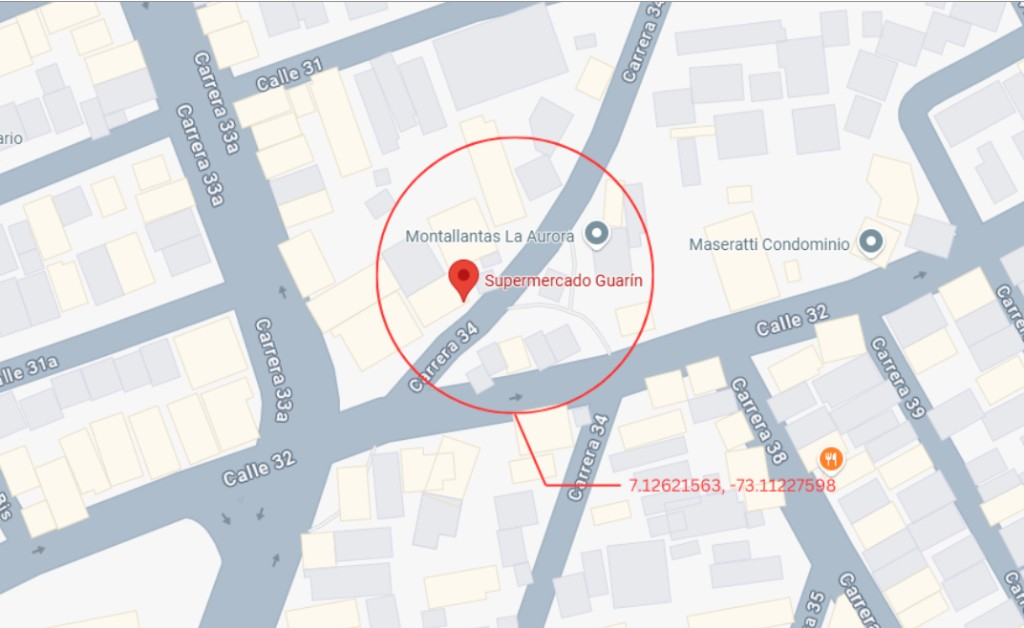
\includegraphics[width=0.95\textwidth]{figuras/figura1_localizacion.png}
    \caption{Localización del proyecto}
    \label{fig:localizacion}
\end{figure}

\section{Caracterización del Circuito 10-502}

La red de conexión corresponde al circuito \textbf{10-502} de la subestación Conucos (13,8~kV), según la información entregada por ESSA. El modelo incluye:

\begin{table}[H]
    \centering
    \caption{Resumen del modelo eléctrico del circuito 10-502}
    \begin{tabular}{lc}
    \toprule
    \textbf{Parámetro} & \textbf{Valor} \\
    \midrule
    Subestación / campo & SE Conucos / 10-502 \\
    Tensión nominal & 13,8 kV \\
    Número de tramos de línea & 215 \\
    Longitud total modelada & 5,061 km \\
    Número de cargas LV & 51 \\
    Suma de cargas modeladas & 7,532 MVA \\
    Demanda máxima en cabecera & 1,683 MVA (12:00 h) \\
    Corriente máxima en cabecera & 70,41 A \\
    Demanda mínima en cabecera & 0,630 MVA (04:00 h) \\
    Punto de conexión AGPE & Nodo 3272966 \\
    \bottomrule
    \end{tabular}
\end{table}

\begin{figure}[H]
    \centering
    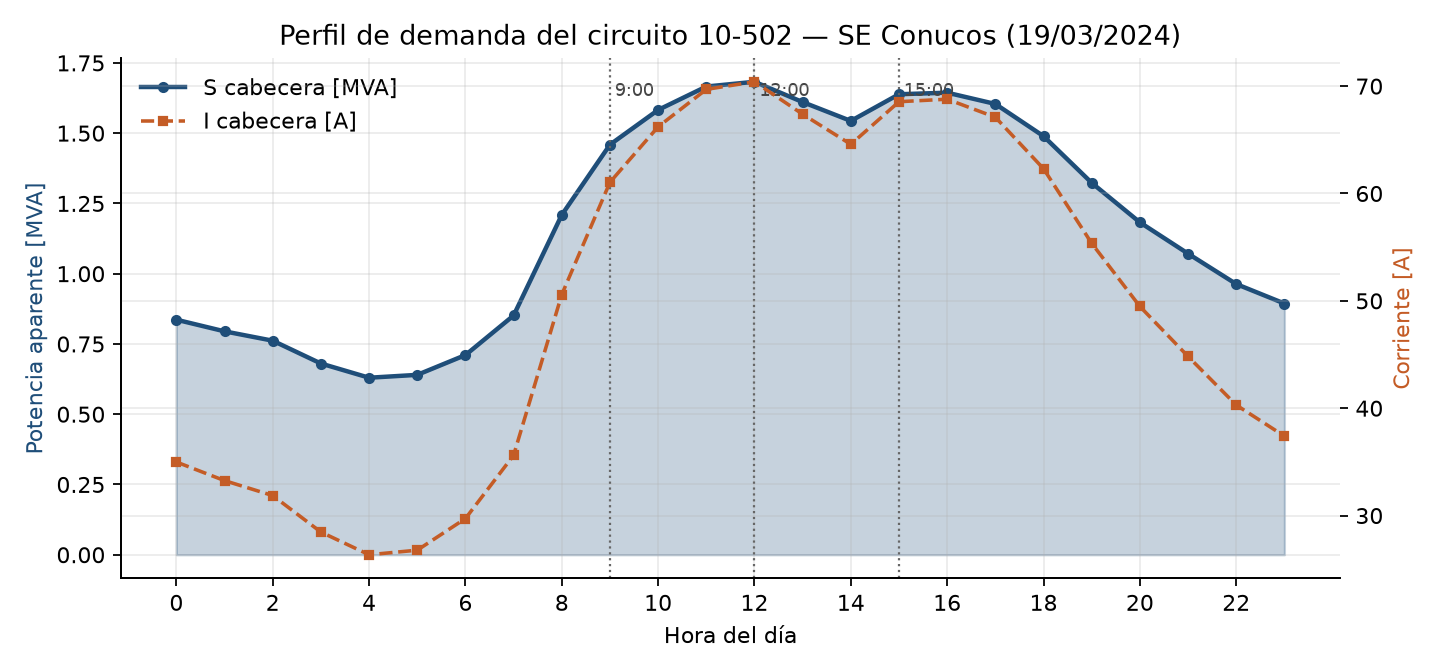
\includegraphics[width=0.95\textwidth]{figuras/fig_demanda_circuito.png}
    \caption{Perfil horario de demanda del circuito 10-502 (19/03/2024)}
    \label{fig:demanda}
\end{figure}

\begin{table}[H]
    \centering
    \caption{Demanda en cabecera del circuito en las horas de análisis}
    \begin{tabular}{cccc}
    \toprule
    \textbf{Hora} & \textbf{I [A]} & \textbf{S [MVA]} & \textbf{Observación} \\
    \midrule
    09:00 & 61,05 & 1,459 & Franja matutina \\
    12:00 & 70,41 & 1,683 & Demanda máxima del día \\
    15:00 & 68,55 & 1,638 & Franja vespertina \\
    \bottomrule
    \end{tabular}
\end{table}

\begin{figure}[H]
    \centering
    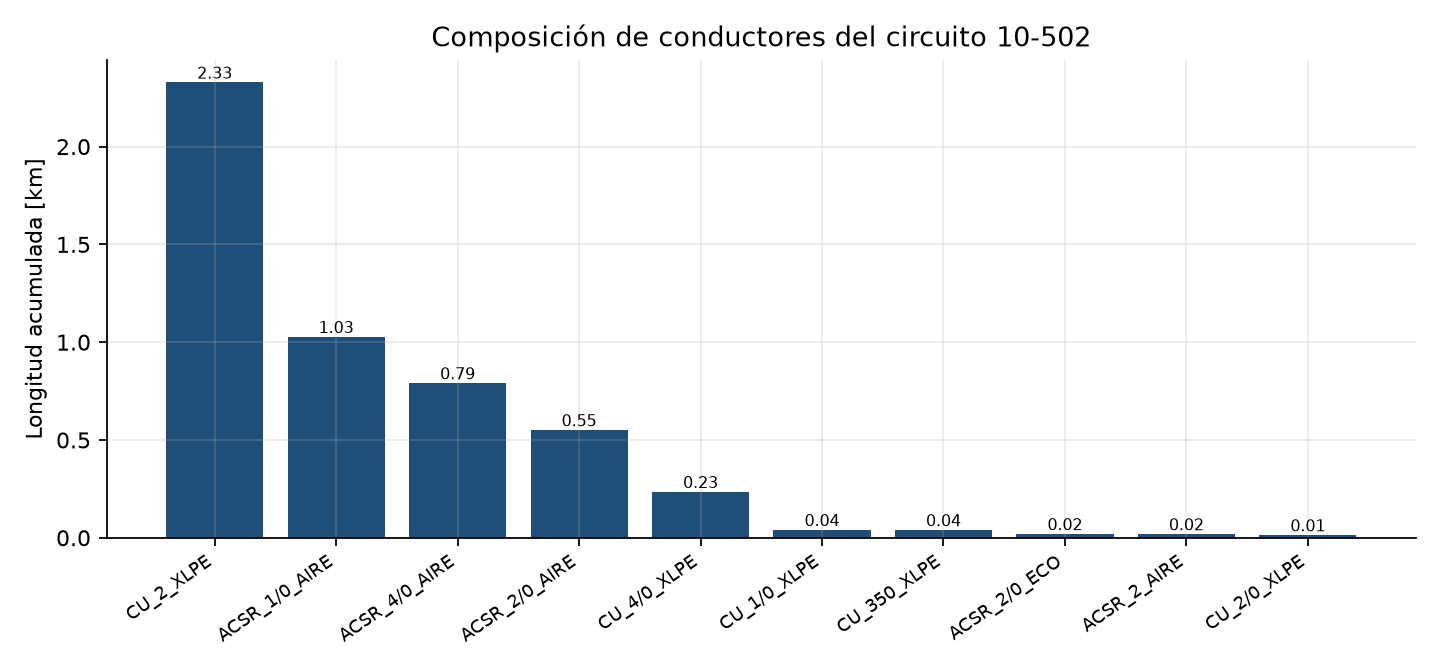
\includegraphics[width=0.95\textwidth]{figuras/fig_conductores.png}
    \caption{Composición de conductores del circuito 10-502}
    \label{fig:conductores}
\end{figure}

\begin{figure}[H]
    \centering
    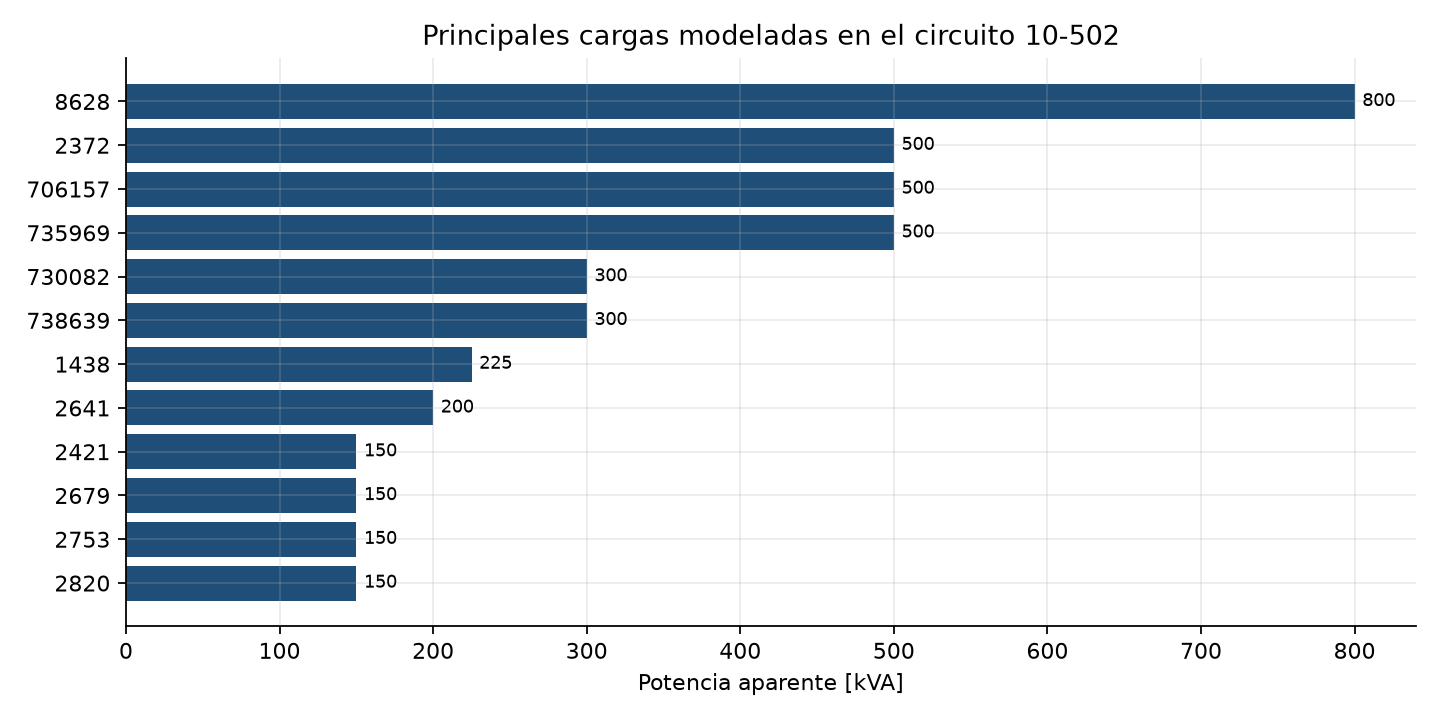
\includegraphics[width=0.95\textwidth]{figuras/fig_top_cargas.png}
    \caption{Principales cargas modeladas (resaltada la carga del POC 3272966)}
    \label{fig:topcargas}
\end{figure}

\section{Punto de Conexión y Ruta Eléctrica}

El apoyo/nodo de conexión del AGPE es el \textbf{3272966}. La acometida MT desde el nodo 3272869 corresponde a la línea \textbf{807675}:

\begin{table}[H]
    \centering
    \caption{Parámetros del tramo de conexión al POC}
    \begin{tabular}{lc}
    \toprule
    \textbf{Parámetro} & \textbf{Valor} \\
    \midrule
    Identificador de línea & 807675 \\
    Terminales & 3272869 -- 3272966A \\
    Conductor & 3F\_15\_CU\_2\_XLPE \\
    Longitud & 0,003 km (3 m) \\
    Corriente nominal & 0,155 kA (155 A) \\
    $R_1$ / $X_1$ & 0,0020 / 0,0013 $\Omega$ \\
    $R_0$ / $X_0$ & 0,0033 / 0,0012 $\Omega$ \\
    \bottomrule
    \end{tabular}
\end{table}

La ruta eléctrica inmediata hacia el POC (desde el ramal cercano) es:

\begin{table}[H]
    \centering
    \small
    \caption{Tramos sucesivos hacia el nodo 3272966}
    \begin{tabular}{cccccc}
    \toprule
    \textbf{Línea} & \textbf{De} & \textbf{A} & \textbf{L [km]} & \textbf{$R_1$ [$\Omega$]} & \textbf{$X_1$ [$\Omega$]} \\
    \midrule
    807671 & 1101455G & 3272567 & 0,0160 & 0,0105 & 0,0068 \\
    807672 & 3272567 & 3272664 & 0,0183 & 0,0120 & 0,0078 \\
    807673 & 3272664 & 3272761 & 0,0077 & 0,0051 & 0,0033 \\
    807674 & 3272761 & 3272869 & 0,0040 & 0,0026 & 0,0017 \\
    807675 & 3272869 & 3272966A & 0,0030 & 0,0020 & 0,0013 \\
    \midrule
    \textbf{Total} & & & \textbf{0,049} & \textbf{0,0322} & \textbf{0,0209} \\
    \bottomrule
    \end{tabular}
\end{table}

\begin{figure}[H]
    \centering
    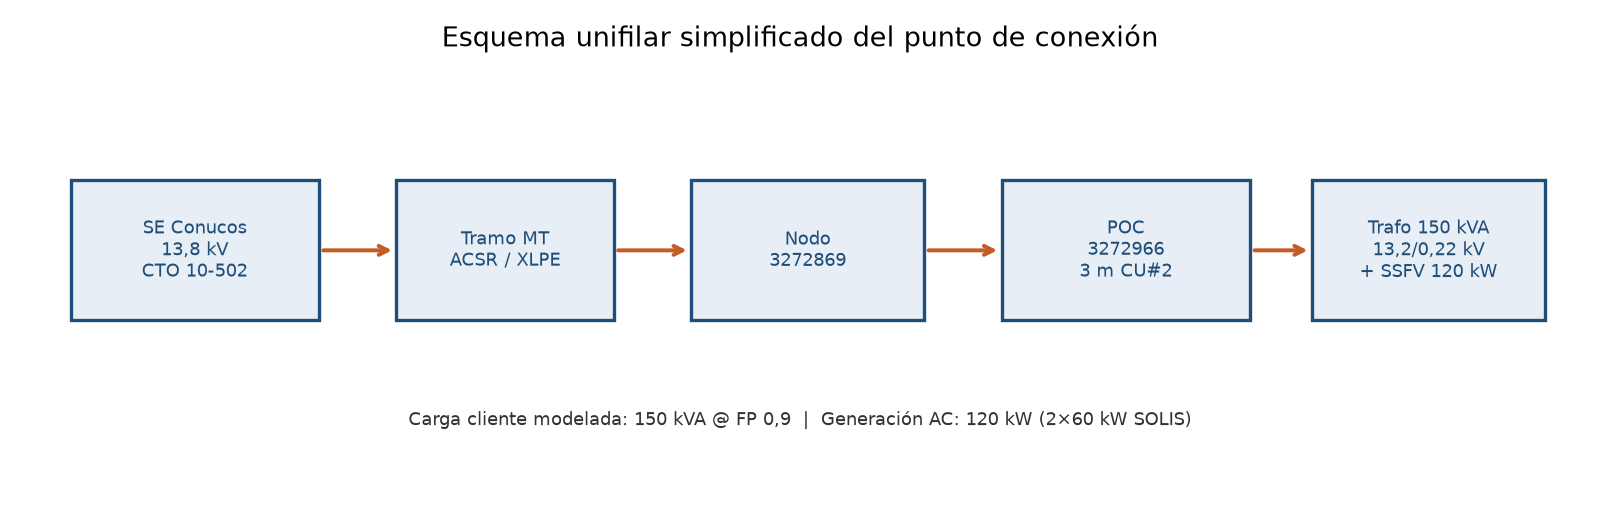
\includegraphics[width=\textwidth]{figuras/fig_esquema_poc.png}
    \caption{Esquema unifilar simplificado del punto de conexión}
    \label{fig:esquema}
\end{figure}

La carga asociada al POC en el modelo del OR es \textbf{730199\_LV\_LOAD}: 0,15~MVA @ FP~0,9 (135~kW / $\approx$65~kVAr).

\section{Parámetros Técnicos de Inversores y Paneles}

\subsection{Inversores}

\begin{table}[H]
    \centering
    \caption{Parámetros técnicos del inversor SOLIS 60K LV 5G}
    \begin{tabular}{lcc}
    \toprule
    \textbf{Parámetro} & \textbf{Valor} & \textbf{Unidad} \\
    \midrule
    Número de inversores & 2 & UND \\
    Tensión máxima de arranque & 195 & VDC \\
    Tensión MPPT en DC entrada & 180 -- 1000 & VDC \\
    Tensión máxima DC entrada & 1100 & VDC \\
    Máxima corriente de entrada & $26 \times 8$ & A DC \\
    Potencia máxima & 69000 & W \\
    Voltaje nominal de salida & 220 & VAC \\
    Frecuencia de salida & 60 & Hz \\
    Corriente de salida & 157,5 & A \\
    Número de fases & 3 & -- \\
    Protección anti-isla & Sí & -- \\
    Factor de potencia & 0,99 & -- \\
    \bottomrule
    \end{tabular}
\end{table}

\subsection{Paneles Fotovoltaicos}

\begin{table}[H]
    \centering
    \caption{Parámetros técnicos de los paneles fotovoltaicos}
    \begin{tabular}{lcc}
    \toprule
    \textbf{Parámetro} & \textbf{Valor} & \textbf{Unidad} \\
    \midrule
    Tipo & \multicolumn{2}{l}{JINKO Monocristalino Mono-facial} \\
    Potencia nominal por panel & 590 & W \\
    Voltaje máximo de salida & 41,05 & VDC \\
    Corriente máxima de salida & 10,83 & A \\
    Eficiencia & 22,84 & \% \\
    Cantidad de paneles & 240 & UND \\
    \bottomrule
    \end{tabular}
\end{table}

\begin{figure}[H]
    \centering
    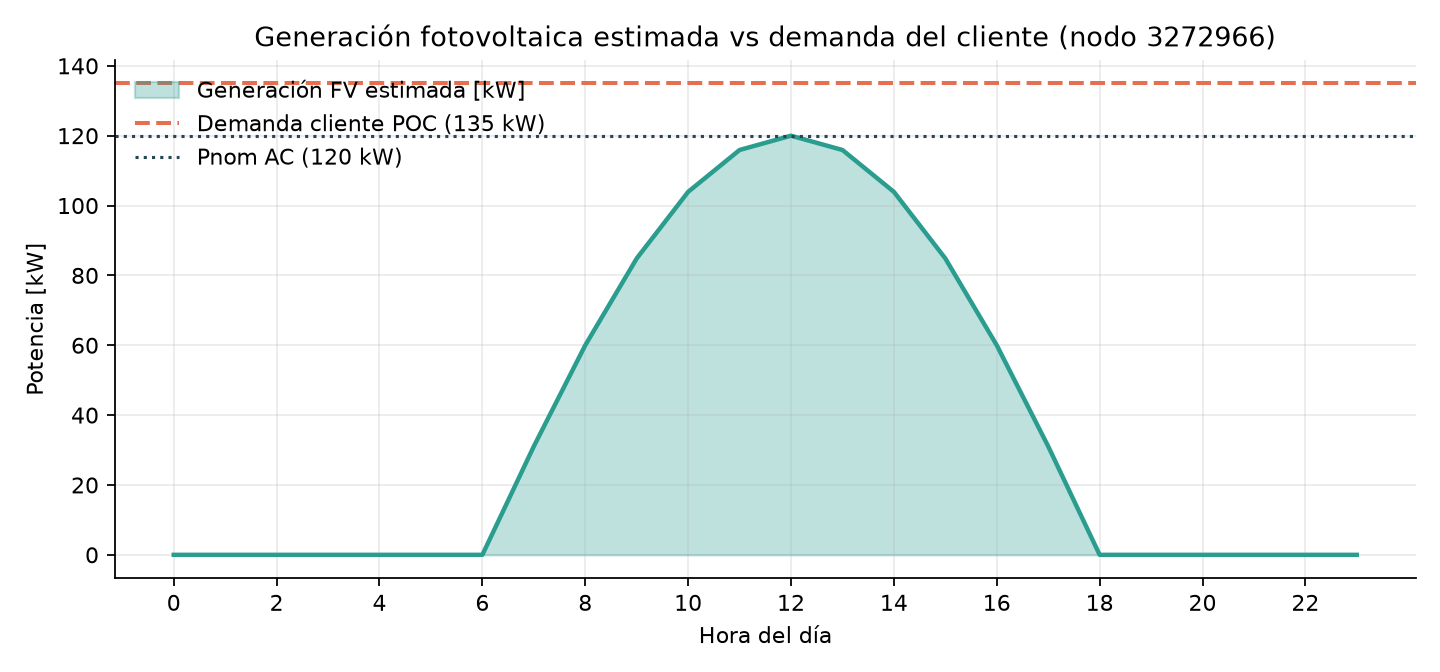
\includegraphics[width=0.95\textwidth]{figuras/fig_gen_vs_demanda.png}
    \caption{Perfil estimado de generación FV vs demanda del cliente en el POC}
    \label{fig:genvsdem}
\end{figure}

\section{Cálculo de Energía Producida}

\subsection{Radiación Solar}

La radiación global anual promedio sobre superficie horizontal en Bucaramanga se estima en 4,7~kWh/m$^2$/día.

\subsection{Ausencia de Sombras}

En la planta en cuestión no se identifica sombreado significativo que afecte la generación del sistema fotovoltaico.

\subsection{Datos de Entrada}

\begin{table}[H]
    \centering
    \caption{Datos de entrada para estimar la energía generada}
    \begin{tabular}{lc}
    \toprule
    \textbf{Parámetro} & \textbf{Valor} \\
    \midrule
    Ubicación del proyecto & Bucaramanga \\
    Coordenadas (LAT, LONG) & 7,12621563, $-$73,11227598 \\
    Capacidad instalada en DC & 141,6 kWp \\
    Capacidad instalada en AC & 120 kW \\
    Tipo de módulo & Premium \\
    Inclinación & 10° \\
    Azimut & 180 \\
    Pérdidas del sistema & 26\% \\
    Eficiencia del inversor & 98,50\% \\
    Relación DC a AC & 1,18 \\
    \bottomrule
    \end{tabular}
\end{table}

\subsection{Fórmula de Energía Producida}

La energía anual estimada se calcula mediante:

\begin{equation}
E_{p,y} = P_{nom}(d.c) \times Irr \times (1 - \text{Losses})
\end{equation}

Donde:
\begin{itemize}
    \item $P_{nom}(d.c)$ = 141,6 kWp
    \item $Irr$ = 1.715,5 kWh/m$^2$/año
    \item Losses = 26\%
\end{itemize}

Con estos parámetros se obtiene una producción estimada del orden de \textbf{179.757~kWh/año}.

\section{Equivalente de Red en SE Conucos}

Para cortocircuito se emplea el equivalente de red en barraje 13,8~kV de la S/E Conucos, reportado por el OR:

\begin{table}[H]
    \centering
    \caption{Niveles de falla en barraje 13,8 kV -- S/E Conucos}
    \begin{tabular}{lcccc}
    \toprule
    \textbf{Tipo de falla} & \textbf{$S_k$ [MVA]} & \textbf{$I_k$ [kA]} & \textbf{$I_p$ [kA]} & \textbf{R/X} \\
    \midrule
    Trifásica & 654,488 & 27,382 & 70,401 & 0,068 \\
    Monofásica a tierra & 239,681 & 30,083 & 77,345 & 0,068 \\
    \bottomrule
    \end{tabular}
\end{table}

\section{Transformador de Conexión}

\begin{table}[H]
    \centering
    \caption{Parámetros técnicos del transformador Serie 21123832-S}
    \begin{tabular}{lcc}
    \toprule
    \textbf{Parámetro} & \textbf{Valor} & \textbf{Unidad} \\
    \midrule
    Potencia & 150 & kVA \\
    Tensión primario / secundario & 13,2 / 220 & kV / V \\
    Impedancia de cortocircuito ($Z_{cc}$) & 4,9 & \% \\
    Grupo de conexión & Dyn5 & -- \\
    \bottomrule
    \end{tabular}
\end{table}

\section{Protección Existente del Circuito}

Según la hoja de protecciones del OR, la bahía del circuito 10-502 dispone de:

\begin{table}[H]
    \centering
    \small
    \caption{Protección principal del circuito 10-502 (SE Conucos)}
    \begin{tabular}{ll}
    \toprule
    \textbf{Parámetro} & \textbf{Valor} \\
    \midrule
    Subestación / bahía & Conuco / CTO 10502 \\
    Tensión & 13,8 kV \\
    RTC / RTP & 60 / 120 \\
    Fabricante / modelo & AREVA / MICOM P142 \\
    Serial & 360 \\
    Funciones & 50, 50N, 51, 51N \\
    Tipo & Protección principal de sobrecorriente \\
    51 (fase) & Pickup 6, dial 0,1, curva IEC VI \\
    50-1 (fase) & Pickup 36, retardo 0 s \\
    51N (tierra) & Pickup 2, dial 0,15, curva IEC VI \\
    50N & Pickup 20 \\
    Recierre 79 & 15/30 s, reset 60 s \\
    \bottomrule
    \end{tabular}
\end{table}
